% Fig. 1(b): the closed loop as simulated (Secs. II-C, IV). All designs
% share actuator, plant and sensor models; the momentum manager (14) only shifts
% the attitude reference, e = theta_e - theta_r. (MPC: law and constraints in
% one optimization, no manager.)
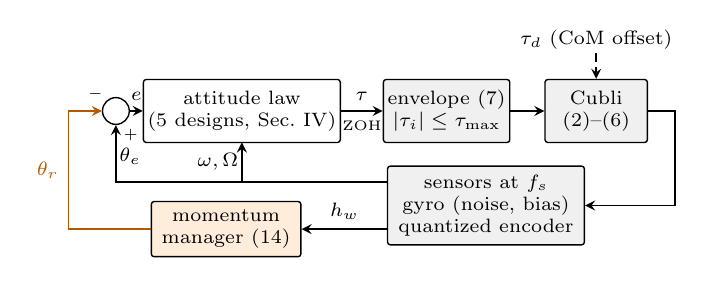
\begin{tikzpicture}[>=stealth, x=1mm, y=1mm, font=\scriptsize, line width=0.5pt,
  blk/.style={draw, rounded corners=1pt, align=center, inner sep=1.5pt},
  flow/.style={->, line width=0.6pt}]
\node[draw, circle, inner sep=0pt, minimum size=3.4mm] (s) at (0,0) {};
\node[blk, minimum width=21mm, minimum height=8mm] (law) at (16,0)
  {attitude law\\(5 designs, Sec.~IV)};
\node[blk, minimum width=16mm, minimum height=8mm, fill=black!6] (act) at (42,0)
  {envelope (7)\\$|\tau_i|\le\tau_{\max}$};
\node[blk, minimum width=13mm, minimum height=8mm, fill=black!6] (plant) at (61,0)
  {Cubli\\(2)--(6)};
\node[blk, minimum width=25mm, minimum height=10mm, fill=black!6] (sens) at (47,-12)
  {sensors at $f_s$\\gyro (noise, bias)\\quantized encoder};
\node[blk, minimum width=19mm, minimum height=7mm, fill=orange!14] (mm) at (14,-15)
  {momentum\\manager (14)};
\node[inner sep=1pt] (dist) at (61,9) {$\boldsymbol\tau_d$ (CoM offset)};
\draw[flow] (s) -- node[above] {$e$} (law);
\draw[flow] (law) -- node[above] {$\boldsymbol\tau$} node[below, font=\tiny] {ZOH} (act);
\draw[flow] (act) -- (plant);
\draw[flow, densely dashed] (dist) -- (plant);
\draw[flow] (plant.east) -- (71,0) -- (71,-12) -- (sens.east);
\draw[flow] (34.5,-9) -- (0,-9) -- node[right, pos=0.45, inner sep=1pt] {$\boldsymbol\theta_e$} (s.south);
\draw[flow] (16,-9) -- node[left, pos=0.5, inner sep=1pt] {$\boldsymbol\omega,\boldsymbol\Omega$} (16,-4);
\draw[flow] (34.5,-15) -- node[above] {$\boldsymbol h_w$} (mm.east);
\draw[flow, orange!70!black] (mm.west) -- (-6,-15) -- node[left, pos=0.5] {$\boldsymbol\theta_r$} (-6,0) -- (s.west);
\node[font=\tiny] at (-2.6,2.2) {$-$};
\node[font=\tiny] at (1.9,-3.1) {$+$};
\end{tikzpicture}
